\section{Introduction}

This labwork explores how two complementary strategies—
\emph{source coding} and \emph{channel error-control coding}—
affect system performance.

A real text sentence is used as the information source.
For the source coding Huffman and ASCII will be compared.
The resulting bit stream is then modulated using QPSK and 16-QAM,
transmitted over additive-white-Gaussian-noise (AWGN) and Rayleigh channels,
and the uncoded bit-error curves serve as baseline performance.

In the second phase, three forward-error-correction options are applied:  
\begin{enumerate}
  \item a $(15,11)$ Hamming block code,
  \item a rate-$1/3$ convolutional code with constraint length $K=7$ (64 states), and
  \item their serial concatenation.
\end{enumerate}

 Figure \ref{fig:RxTx} shows the complete system.

\begin{figure}[H]
  \centering
  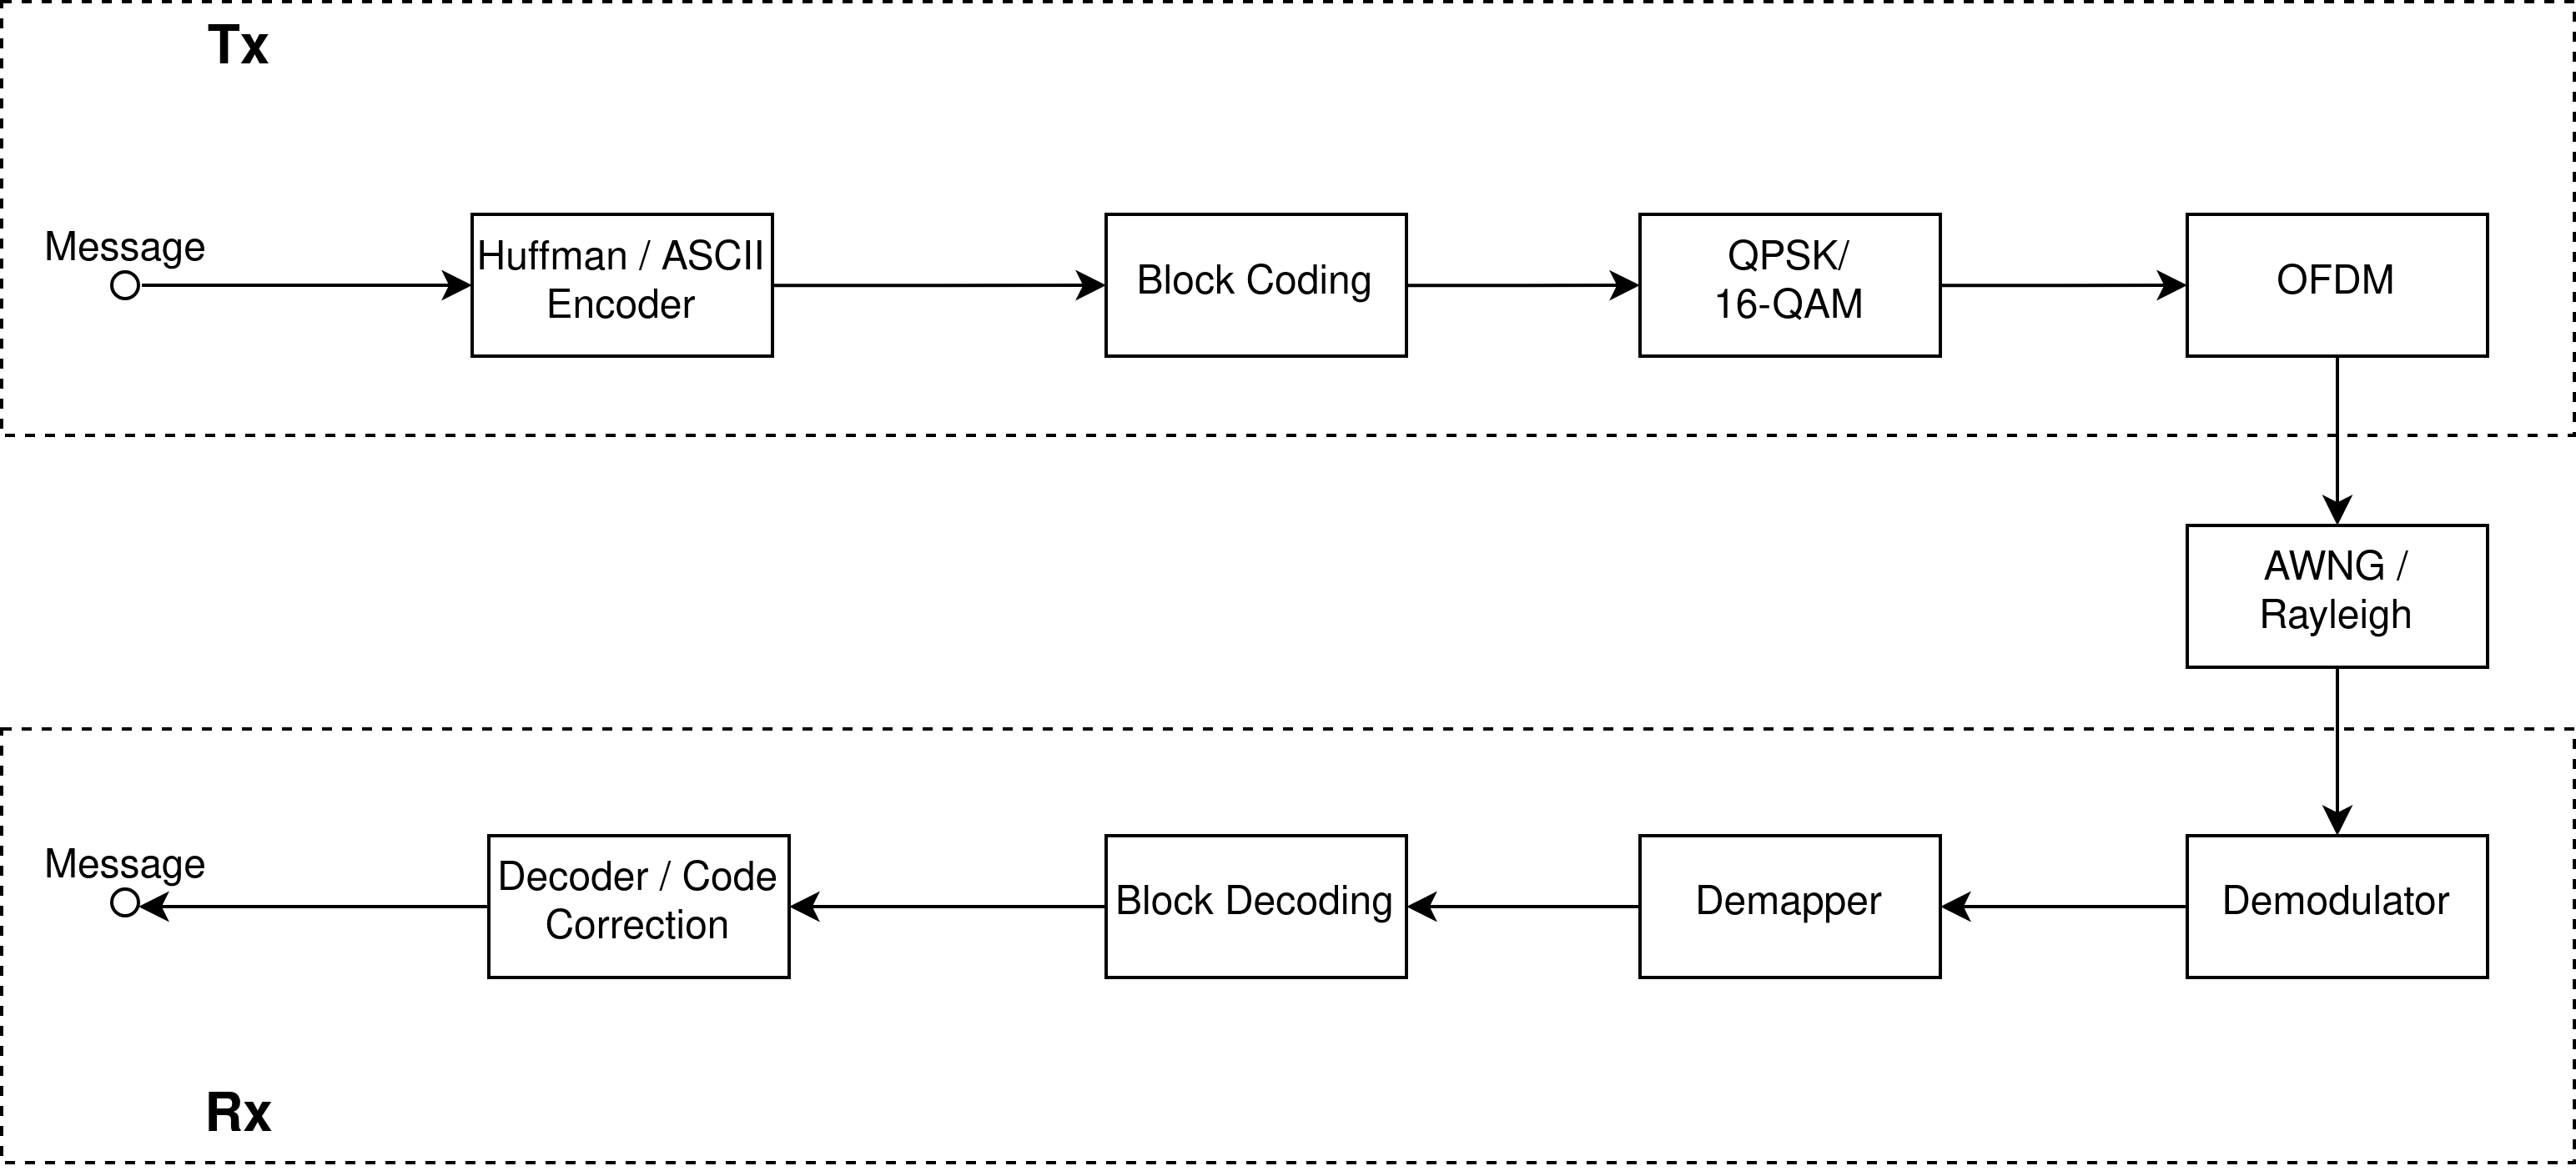
\includegraphics[width=0.9\textwidth]{Images/BlockDiagram.png}
  \caption{Receiver and Transmitter block diagram.}
  \label{fig:RxTx}
\end{figure}


For each configuration more than one million bits are simulated, and the
bit-error rate (BER) and frame-error rate (FER) are measured as functions
of the energy-per-bit to noise ratio $E_b/N_0$.  
\textcolor{red}{Quando tiver feito verificar isto}
These results are translated into \emph{effective information throughput}
and \emph{re-transmission probability}, allowing a quantitative study of
the trade-offs among compression gain, coding gain and spectral efficiency.

\textcolor{red}{Quando tiver feito verificar isto}
The laboratory therefore demonstrates how carefully chosen source and
channel codes enable high-capacity transmission while meeting a stringent
reliability target (FER $<10^{-5}$) characteristic of 5G and other
advanced networks.
